\documentclass[11pt,letterpaper]{article}
\usepackage[utf8]{inputenc}
\usepackage[T1]{fontenc}
\usepackage[spanish]{babel}
\usepackage{amsmath,amssymb}
\usepackage{amsfonts}
\usepackage{amssymb}
\usepackage{graphicx}
\usepackage{lmodern}
\usepackage{xspace}
\usepackage{multicol}
\usepackage{hyperref}
\usepackage{float}
\usepackage{hyperref}
\usepackage{color}
\usepackage{framed}

%\usepackage[colorlinks=true, linkcolor=black, urlcolor=blue, pdfborder={0 0 0}]{hyperref}

\usepackage[left=2cm,right=2cm,top=2cm,bottom=2cm]{geometry}

\newcommand{\X}{\mathbb{X}}
\newcommand{\x}{\mathbf{x}}
\newcommand{\Y}{\mathbf{Y}}
\newcommand{\y}{\mathbf{y}}
\newcommand{\xbarn}{\bar{x}_n}
\newcommand{\ybarn}{\bar{y}_n}
\newcommand{\paren}[1]{\left( #1 \right)}
\newcommand{\llaves}[1]{\left\lbrace #1 \right\rbrace}
\newcommand{\barra}{\,\vert\,}
\newcommand{\mP}{\mathbb{P}}
\newcommand{\mE}{\mathbb{E}}

\newcommand{\abs}[1]{\left\vert #1 \right\vert}
\newcommand{\muv}{\boldsymbol{\mu}}
\newcommand{\mcov}{\boldsymbol{\Sigma}}
\newcommand{\vbet}{\boldsymbol{\beta}}
\newcommand{\veps}{\boldsymbol{\epsilon}}
\newcommand{\mC}{\mathbf{C}}
\newcommand{\ceros}{\boldsymbol{0}}
\newcommand{\mH}{\mathbf{H}}
\newcommand{\ve}{\mathbf{e}}
\newcommand{\avec}{\mathbf{a}}
\newcommand{\res}{\textbf{RESPUESTA}\\}

\newcommand{\fin}{$\blacksquare.$}
\newcommand{\finf}{\blacksquare.}

\newtheorem{thmt}{Teorema:}
\newtheorem{thmd}{Definición:}
\newtheorem{thml}{Lema:}
\newcommand{\intim}{\int_{-\infty}^\infty}
\newcommand{\fx}{f_X(x)}
\newcommand{\fy}{f_Y(y)}

\begin{document}
\begin{table}[ht]
\centering
\begin{tabular}{c}
\textbf{Maestría en Computo Estadístico}\\
\textbf{Inferencia Estadística} \\
\textbf{Tarea 4}\\
\today \\
\emph{Enrique Santibáñez Cortés}\\
Repositorio de Git: \href{https://github.com/Enriquesec/Inferencia_Estad-stica/tree/master/Tareas/Tarea_4}{Tarea 4, IE}.
\end{tabular}
\end{table}
Escriba de manera concisa y clara sus resultados, justificando los pasos necesarios. Serán descontados puntos de los ejercicios mal escritos y que contenga ecuaciones sin una estructura gramatical adecuada. Las conclusiones deben escribirse en el contexto del problema. Todos los programas y
simulaciones tienen que realizarse en R.
%Problema 1
%------------------------------------------------------------------------------------------------------%
%------------------------------------------------------------------------------------------------------%
%------------------------------------------------------------------------------------------------------

1. Sea $X$ una v.a continua cuya función de distribución $F$ es estrictamente creciente. El Teorema
de la Transformación Integral nos dice que $Y=F(X)$ tiene distribución Uniforme(0, 1).\\

a) Sea $U\sim Uniforme(0, 1)$ y $X'=F ^{-1}(U)$. Muestre que $X' \sim F$.

\res Como $U$ tiene una distribución $Unif(0,1)$, esto implica que $F_U(u)=u$ (por definición de la función acumulada de una distribución uniforme). Entonces tenemos que 
\begin{align*}
F_{X'}(x')=\mP(X'\leq x')=\mP(F^{-1}(U)\leq x')= \mP(U\leq F(x'))= F_U(F(x'))=F(x').
\end{align*}
Por lo tanto, $X'\sim F.$

%Problema 2
%------------------------------------------------------------------------------------------------------%
%------------------------------------------------------------------------------------------------------%
%------------------------------------------------------------------------------------------------------%
2. Sea A el triángulo de vértices (0, 0), (0, 1), (1, 0) y suponga que $X, Y$ tiene una densidad conjunta uniforme en el triángulo. (a) Halle las distribuciones marginales de $X, Y \ \text{y}\ Z =X + Y$ . (b) ¿Son $X$ y $Y$ independientes? ¿Por qué?

\res Por como esta descrita la densidad conjunta de $X,Y$ podemos escribirla como 
\begin{align*}
f(x,y)=\left\{\begin{array}{cc}
2,& 0\leq x\leq 1, x\leq y\leq 1\\
0,& \text{otro caso}.
\end{array} .\right.
\end{align*}
Validamos que efectivamente cumpla las condiciones de densidad conjunta, observemos que se cumple que $f(x,y)\geq 0, \ \forall (x,y).$ y además que integra 1:
\begin{align*}
\intim \intim f(x,y)dydx=\int_0^1 \int_x^1 2 dydx=\int_0^1 2(1-x) dx=\left.2x-\frac{2x^2}{2}\right|_0^1=1.
\end{align*}
La definición de distribuciones marginales:
\begin{framed}
    \begin{thmd} \label{marginales}
	Las distribuciones marginales de v.a continuas $X$ y $Y$, denotadas por $f_X(x)$ y $f_Y(y),$ se definen como
	\begin{align*}
	f_X(x) = \intim f(x,y)dy,\\
	\text{y}\\
	f_Y(y)=\intim f(x,y)dx.
	\end{align*}
    \end{thmd}
\end{framed}
Entonces \textbf{a) las marginales son}:
\begin{align*}
f_X(x)=\intim f(x,y)dy =\int_x^1 2 dy=\left. y\right|_{0}^1=2(1-x).\\
f_Y(y)=\intim f(x,y)dx=\int_y^1 2 dx=\left. x\right|_{0}^1=2(1-y),
\end{align*} es decir,
\begin{align*}
f_X(x)=\left\{\begin{array}{cc}
2(1-x) & 0\leq x\leq 1\\
0 & \text{en otro caso.}
\end{array} \right.\ \ \ \ \text{y} \ \ \ f_Y(y)=\left\{\begin{array}{cc}
2(1-y) & 0\leq y\leq 1\\
0 & \text{en otro caso.}
\end{array} \right.
\end{align*} 
\textbf{La marginal de $Z=X+Y$ se entrega en la próxima tarea.}\\

Ocupando la siguiente definición (vista en clase):
\begin{framed}
    \begin{thmd} \label{independencia}
    Dos variables aleatorias continuas se dice que son \textbf{independientes} si su distribución conjunta se puede expresar como el producto de sus marginales.
    $$f(x,y)=f_X(x)f_Y(y).$$
    \end{thmd}
\end{framed} 
Lo anterior es equivalente a decir que si la distribución conjunta no se puede expresar como el producto de sus marginales entonces no es independientes (equivalencia lógica). Entonces observemos que:
\begin{align*}
f(x,y)=2\neq 2(1-x)\cdot 2(1-y)=\fx \fy .
\end{align*}
Por lo tanto, \textbf{b) podemos concluir que $X$ y $Y$ no son independientes por que el producto de sus marginales no es la conjunta.}\ \ \  \fin
 
%Problema 3
%------------------------------------------------------------------------------------------------------%
%------------------------------------------------------------------------------------------------------%
%------------------------------------------------------------------------------------------------------
3. Halle la densidad condicional de $X|Y=y$ si $(X,Y)$ tiene densidad conjunta \begin{align*}
f_{X,Y}(x,y)=\frac{1}{y}\exp \left(-\frac{x}{y}-y \right) \ \text{para} \ x,y>0.
\end{align*} 
También calcule $\mE(X|Y=y)$.

\res Recordemos la definición de distribución condicional:
\begin{framed}
    \begin{thmd} \label{distribucion_condicional}
    Las distribuciones condicionales de $X|Y=y$ y $Y|X=x$ denotadas por $f_{X|y}(x)$ y $f_{Y|x}(y)$ se definen de la siguiente forma. Para cada valor de $y$ 
    \begin{align*}
f_{X|y}(x)=\frac{f(x,y)}{f_Y(y)}.
\end{align*}
Es un función de densidad en $X$. Sus valores pueden depender (en el sentido de función matemática, de $y$, pero como este valor es dado, no representa un factor aleatorio). Análogamente, para cada valor $x$
	   \begin{align*}
	f_{Y|x}(y)=\frac{f(x,y)}{f_X(x)}.
	\end{align*}
    \end{thmd}
\end{framed} 

Entonces calculemos la función de densidad marginal de $Y$ en este problema es:
\begin{align*}
f_Y(y)=\int_{-\infty}^\infty f(x,y)dx=\int_{0}^\infty  \frac{1}{y}\exp \left(-\frac{x}{y}-y \right)dx=\frac{1}{y}\int_{0}^\infty \exp \left(-\frac{x}{y}-y \right)dx
\end{align*}
ocupando un cambio de variable $m=-\frac{x}{y}-y\Rightarrow dm=-\frac{1}{y}dx$, entonces
\begin{align*}
f_Y(y)&=\frac{1}{y}\int_{0}^\infty \exp \left(-\frac{x}{y}-y \right)dx=\frac{1}{y}\int_{0}^\infty \exp \left(m \right)(-y\ dm)=-\exp(m)=-\exp\left.\left(-\frac{x}{y}-y\right)\right|_{x=0}^\infty\\ \\ 
&=\exp(-y).
\end{align*}
Es decir, la marginal de $Y$ es:
$$f_Y(y)=\exp(-y), \ \ y>0.$$
Entonces la distribución conjunta de $X|Y=y$ es:
\begin{align*}
f_{X|y}(x)=\frac{f(x,y)}{f_Y(y)}=\frac{\frac{1}{y}\exp\left(-\frac{x}{y}-y \right) }{\exp(-y)}=\frac{1}{y}\exp\left(\frac{x}{y}-y +y\right)=\frac{1}{y}\exp\left(\frac{x}{y}\right).
\end{align*}
Por lo tanto:
\begin{align*}
\mE(X|Y=y) =\int_{-\infty}^\infty x f_{X|y}(x)dx=\int_{0}^\infty \frac{x}{y}\exp\left(\frac{x}{y}\right). dx.
\end{align*}
Si observamos, es la esperanza de una variable que se distribuye como una exponencial con parámetro $\frac{1}{y}.$ Entonces, como sabemos que la esperanza de una variable poisson con parámetro $\lambda$ es $\frac{1}{\lambda}.$ Entonces \textbf{podemos concluir que esperanza condicional es}:
\begin{align*}
\mE(X|Y=y)= y.\ \ \ \finf
\end{align*}

%Problema 4
%------------------------------------------------------------------------------------------------------%
%------------------------------------------------------------------------------------------------------%
%------------------------------------------------------------------------------------------------------%

4. Sea $Y\sim \exp(\theta)$ y dado $Y=y$, X tiene distribución de Poisson de media $y$. Encuentre la ley de $X$.

\res Veamos que la densidad de $Y$ es 
\begin{align*}
\fy = \theta e^{-\theta y}. \ \ y>0.
\end{align*}
Y podemos ver que la densidad condicional de $X$ dado $Y=y$ es
\begin{align*}
f_{X|y}(x)= \frac{y^xe^{-y}}{x!}. \ x>0.
\end{align*}
Entonces usando la ley de probabilidad total tenemos que 
\begin{align*}
\fx&=\int_0^\infty f_{X|y}(x)f_Y(y)dy = \int_0^\infty \frac{y^xe^{-y}}{x!}  \theta e^{-\theta y} dy = \theta\int_0^\infty \frac{y^x e^{-(1+\theta)y}}{x!}dy
\end{align*}
haciendo un cambio de variable tenemos que $m=(1+\theta)y\Rightarrow dm=(1+\theta),$ entonces
\begin{align*}
\theta\int_0^\infty \frac{(m/(1+\theta))^x e^{-m}}{x!}dm= \frac{\theta}{(1+\theta)^{x+1}}\int_0^\infty \frac{m^x e^{-m}}{x!}dy=\frac{\theta}{(1+\theta)^{x+1}}.
\end{align*}
Por lo tanto, tenemos que
\begin{align*}
\fx = \frac{\theta}{(1+\theta)^{x+1}}, \ \ x=0,1\cdots
\end{align*}
Si hacemos un cambio de variable $p=\frac{1}{1+\theta}$, tenemos que lo anterior es igual a 
\begin{align*}
\fx = \frac{\theta}{(1+\theta)^{x+1}}=(1-p)p^n.
\end{align*}
Entonces podemos observar que $X\sim Geo(p).$ \ \ \ \ \fin

%Problema 5
%------------------------------------------------------------------------------------------------------%
%------------------------------------------------------------------------------------------------------%
%------------------------------------------------------------------------------------------------------%
5. Sea $(X, Y)$ un vector aleatorio con la siguiente densidad
\begin{align*}
f(x,y)=\left\{\begin{matrix}
\pi^{-1} & x^2+y^2\leq 1\\
0 & x^2+y^2>1
\end{matrix} \right.
\end{align*} 
Demuestre $X$ y $Y$ no están correlacionadas, pero que no son independientes.

\res Observemos que $X$ y $Y$ pueden tomar cualquier valor en el intervalo $[-1,1]$, por lo que podemos decir que son variables continuas. Entonces ocupando la definición de densidades marginales \ref{marginales}, las densidades marginales son:
\begin{align*}
\fy=\int_{-\sqrt{y^2-1}}^{\sqrt{y^2-1}}\pi^{-1} dx=\left.x\pi^{-1} \right|_{-\sqrt{y^2-1}}^{\sqrt{y^2-1}}=2\sqrt{y^2-1}\pi^{-1}, \ -1\leq y \leq 1.\\
\fx=\int_{-\sqrt{x^2-1}}^{\sqrt{x^2-1}}\pi^{-1} dy=\left.y\pi^{-1} \right|_{-\sqrt{x^2-1}}^{\sqrt{x^2-1}}=2\sqrt{x^2-1}\pi^{-1}, \ -1\leq x \leq 1,
\end{align*}
es decir, 
\begin{align*}
\fx=\left\{ \begin{array}{cc}
2\sqrt{x^2-1}\pi^{-1} & -1\leq x \leq 1.\\
0 & \text{en otra caso.}
\end{array} \right., \ \text{y}\ \fy=\left\{ \begin{array}{cc}
2\sqrt{y^2-1}\pi^{-1} & -1\leq y \leq 1.\\
0 & \text{en otra caso.}
\end{array} \right.
\end{align*}
Ocupando el teorema \ref{independencia} podemos observar que
\begin{align*}
f(x,y)=\pi^{-1}\neq 2\sqrt{x^2-1}\pi^{-1} 2\sqrt{y^2-1}\pi^{-1} =\fx \fy.
\end{align*}
\textbf{Por lo que podemos concluir que $X$ y $Y$ no son independientes.}\\ 

Ahora calculemos las siguientes esperanzas $\mE[X], \mE[Y], \mE[XY]:$
\begin{align*}
\mE[X]=\intim x \fx dx = \int_{-1}^1 2x\sqrt{x^2-1}\pi^{-1}dx
\end{align*}
ocupando un cambio de variable $m=x^2-1\Rightarrow dm =2xdx$, entonces 
\begin{align*}
\int 2x\sqrt{x^2-1}\pi^{-1}dx=\pi^{-1}\int \sqrt{m} dm=\pi^{-1}\frac{2m^{3/2}}{3} = \frac{2(x^2-1)^{3/2} \pi^{-1}}{3}.
\end{align*}
Por lo que 
\begin{align*}
E[X]=\left. \frac{2(x^2-1)^{3/2} \pi^{-1}}{3} \right|_{-1}^1=\frac{2(1^2-1)^{3/2} \pi^{-1}}{3}-\frac{2(1^2-1)^{3/2} \pi^{-1}}{3}=0.
\end{align*}
Ahora,
\begin{align*}
\mE[Y]=\intim y \fy dy = \int_{-1}^1 2y\sqrt{y^2-1}\pi^{-1}dy
\end{align*}
ocupando un cambio de variable $m=y^2-1\Rightarrow dm =2ydy$, entonces 
\begin{align*}
\int 2y\sqrt{y^2-1}\pi^{-1}dy=\pi^{-1}\int \sqrt{m} dm=\pi^{-1}\frac{2m^{3/2}}{3} = \frac{2(y^2-1)^{3/2} \pi^{-1}}{3}.
\end{align*}
Por lo que 
\begin{align*}
E[Y]=\left. \frac{2(y^2-1)^{3/2} \pi^{-1}}{3} \right|_{-1}^1=\frac{2(1^2-1)^{3/2} \pi^{-1}}{3}-\frac{2(1^2-1)^{3/2} \pi^{-1}}{3}=0.
\end{align*}
Y por último:
\begin{align*}
\mE[XY]=\intim\intim xy f(x,y) dx dy = \int_{-1}^1 \int_{-\sqrt{x^2-1}}^{\sqrt{x^2-1}} xy\pi^{-1}dydx=\int_{-1}^1 x\pi^{-1}\left( \int_{-\sqrt{x^2-1}}^{\sqrt{x^2-1}} y\right) dydx \\ \\
=\int_{-1}^1 x\pi^{-1}\left(\left. \frac{y^2}{2}\right|_{-\sqrt{x^2-1}}^{\sqrt{x^2-1}} \right) dx =\int_{-1}^1 x\pi^{-1}\left( \frac{{\sqrt{x^2-1}}^2-\sqrt{x^2-1}^2}{2} \right) dx \int_{-1}^1 x\pi^{-1}\left(0 \right) dx =0.
\end{align*}
Entonces ocupando los resultados anteriores tenemos que 
\begin{align*}
Cov(X,Y)=\mE[(X-\mE(X))(Y-\mE(Y))]=\mE(XY)-\mE(X)\mE(Y)=0-0=0.
\end{align*}
Lo anterior implica que $\rho=0.$ \textbf{Y por lo tanto, podemos concluir que las $X$ y $Y$ no están correlacionadas.} \ \ \ \fin

Este es un claro ejemplo de que si $Cov(X,Y)=0$, no necesariamente es cierto que las variables sean independientes, simplemente dice que no hay dependencia lineal, pero puede ser otro tipo de dependencia, que en el sentido contrario si es cierto. 
%Problema 6
%------------------------------------------------------------------------------------------------------%
%------------------------------------------------------------------------------------------------------%
%------------------------------------------------------------------------------------------------------%

6. \textbf{Se entrega en la próxima tarea.} \\

%Problema 7
%------------------------------------------------------------------------------------------------------%
%------------------------------------------------------------------------------------------------------%
%------------------------------------------------------------------------------------------------------%

%Problema 8
%------------------------------------------------------------------------------------------------------%
%------------------------------------------------------------------------------------------------------%
%------------------------------------------------------------------------------------------------------%
8. Supongamos que se desea estudiar un número, $n$, grande de muestras de sangre para tratar de detectar una enfermedad rara en cada una de las muestras. Si cada muestra es analizada individualmente, se requieren $n$ pruebas. Supongamos que cada muestra se divide a la mitad y que de cada muestra se selecciona una de las mitades, las que se usan para crear una mezcla de todas ellas (i.e. se juntan en una sola muestra). Si la prueba es suficientemente sensitiva, esta mezcla puede examinarse y, si tal prueba sale negativa, no se requieren hacer mías pruebas y solo se necesita una (no hay enfermos en la muestra). Si la prueba de la mezcla es positiva, cada una de las mitades reservadas de la muestras (las mitades no mezcladas) pueden ser analizadas individualmente. En dicho caso, se necesitan un total de $n+ 1$. Así, si la enfermedad es rara, es posible que se puedan lograr algunos ahorros a través de este método
de analizar en grupo.\\
Generalicemos el esquema anterior y supongamos que las $n$ muestras primero se agrupan en $m$ grupos de tamaño $k$ (muestras); es decir, $n = mk$. Cada grupo se prueba con el método de grupo que se explico en el párrafo anterior; si un grupo sale positivo, cada individuo en el grupo es analizado individualmente. Si $X_i$ es el número de pruebas que se hacen en el $i-$ésimo grupo, el número total de pruebas que se hacen es $N =\sum_{i=1}^m Xi$. Sea $p$ la probabilidad de
que un individuo cualquiera salga negativo en la prueba. Calcule la esperanza de $N$. ¿Por qué es importante que la enfermedad sea rara? Hint: Lea cuidadosamente el ejercicio. Note que la prueba de una muestra resulta en una v.a. $Bernoulli(p)$.

\res Veamos como se distribuye $X_i,$ solo puede tomar dos valores 1 o $k+1$. La probabilidad de que $X_i$ sea 1 es $p^k$, ya que es la probabilidad de la todos los $k$ individuos en el grupo $i$ salen negativos y sabiendo que $p$ es la probabilidad de que un individuo cualquiera salga negativo, y como la probabilidad de que un individuo salga negativo es independiente a que otro individuo salga negativo se concluye que es $p^k$. Ahora, La probabilidad de que $X_i$ sea $k+1$ es $1-p^k$, ya que es la probabilidad de que salgan algún positivo en el grupo $i$ pero es equivalente al complemento de que todos salgan negativos. Por lo tanto, tenemos que la función de densidad de $X_i$ es:
\begin{align*}
f(x_i)=\left\{\begin{array}{cc}
p^k & x_i=1\\
1-p^k & x_i=k+1. 
\end{array} \right.
\end{align*}
Ahora, por como esta definidos los $X_i$ suponemos que son independientes. Entonces tenemos que
\begin{align*}
\mE[N]&=\mE\left[\sum_{i=1}^m Xi\right]= \sum_{i=1}^m \mE[X_i]=\sum_{i=1}^m 1\cdot p^k+(1-p^k)*(k+1)=\sum_{i=1}^m p^k+k+1-kp^k-p^k\\
&=\sum_{i=1}^m (k+1-kp^k)=m(k+1-kp^k).
\end{align*}
Si la enfermedad es rara eso implica que $p^k$ sea pequeña, por lo que en teoría $p^k>1-p^k$, es decir, sería más probable hacer una prueba que $k+1$ pruebas. Entonces en términos económicos y de tiempos, la metodología expuesta es muy eficaz y más óptima que analizar siempre todas las muestras por separados.  \ \ \ \fin

\textbf{Honours problems}

1. Sea $X$ una v.a continua con segundo momento finito. Demuestra que la mediana $M(X)$ de $X$ satisface

\begin{align*}
|M(X)-E(X)|\leq (Var(X))^{1/2}.
\end{align*}

Hint: Use los honour problems de la tarea anterior.

\res Recordemos el siguiente teorema (visto en clase). 
\begin{framed}
    \begin{thmt}(Desigualdad de Jensen) \label{desigualdad_de_Jensen}
    Si $X$ es una v.a con primer momento finito y $g$ es convexa, entonces 
    $$E(g(X))\geq g(E(X)).$$
    \end{thmt}
\end{framed} 

Si definimos a $g(x)=(|x-c|)^2\Leftrightarrow g(x)=(x-c)^2,$  observemos que:
\begin{align*}
g'(x)=2x-2c \ \ \text{y} \ \ g''(x)=2.
\end{align*}
Entonces como $g''(x)>0$ podemos decir que $g(x)$ es convexa. Ocupando el teorema \ref{desigualdad_de_Jensen} tenemos que 
\begin{align} \label{desigualdad}
\mE(|X-c|^2)\geq |c-\mE(X)|^2.
\end{align}
Observemos que cuando $c=\mE(X)$
\begin{align*}
E(|x-\mE(X)|^2)=Var(X).
\end{align*}
Ocupando lo demostrado en la tarea 3, podemos decir que cuando $c=M(X)$ se minimiza $\mE(|X-c|^2),$ por lo que se cumple que
\begin{align*}
Var(X)=\mE(|x-\mE(X)|^2)\geq \mE(|X-M(X)|^2)
\end{align*}
Y por lo tanto, ocupando \ref{desigualdad}:
\begin{align*}
Var(X)=\mE(|x-\mE|^2)\geq \mE(|X-M(X)|^2) &\geq (|M(X)-\mE(X)|^2)\ \Rightarrow \\ \\
(Var(X))^{1/2}&\geq |M(X)-\mE(X)|\ \ \ \finf
\end{align*}

\textbf{Ejercicios de las notas:}

1. Se quiere verificar la programación del tiempo que debe durar la luz verde en un semáforo que se encuentra en una cierta intersección, con vuelta a la izquierda. Como no se tiene información al respecto, se envía a un estudiante graduado a hacer observaciones sobre el número de carros $X$
y el número de camiones $Y$ que llegan en un ciclo (entre verde y verde); y con esto se construye la tabla de distribuciones conjunta. Se plantean una serie de preguntas y con ello confirmas qué tan eficiente fue el ciclo planeado. Los resultados fueron los siguientes
\begin{figure}[H]
\centering
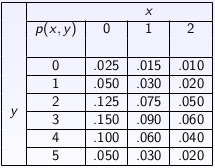
\includegraphics[scale=1]{semaforo.png}
\end{figure}
\begin{enumerate}
\item Verifica que es una tabla válida de probabilidades conjuntas.

\res Observemos que todas las probabilidades son menores a 1 y mayores a 0, por lo que si cumple que $p(x,y)>0.$ Ahora validemos que la suma de todas las probabilidades conjuntas sumas 1:
\begin{align*}
\sum_{i=0}^5 \sum_{j=0}^2 p(X=j,Y=i)&= 0.025+0.050+0.125+0.150+
0.100+0.050+0.015+0.030+0.075+\\
&\ \ \ \ 0.090+0.060+0.030+0.010+ 0.020+0.050+0.060+0.040+0.020\\
&=1
\end{align*}
Por lo tanto si cumple los dos supuestos para ser una probabilidad conjunta. 

\item Calcula las distribuciones marginales para carros y camiones.

\res Por definición \ref{marginales} tenemos que:
\begin{align*}
p(x)&= \sum_{i=0}^5 p(x,Y=i) \Rightarrow \left\{\begin{array}{cc}
0.025+0.050+0.125+0.150+
0.100+0.050=\textbf{0.5} & \text{si} \ x=0\\
0.015+0.030+0.075+0.090+0.060+0.030=\textbf{0.3} & \text{si} \ x=1\\
0.010+ 0.020+0.050+0.060+0.040+0.020= \textbf{0.2} & \text{si} \ x=2
\end{array} \right. \ \text{y} \\ \\
p(y)&= \sum_{j=0}^2 p(X=j,y) \Rightarrow \left\{\begin{array}{cc}
0.025+0.015+0.010=\textbf{0.05} & \text{si} \ y=0\\
0.050+0.030+0.020=\textbf{0.10} & \text{si} \ y=1\\
0.125+0.075+0.050= \textbf{0.25} & \text{si} \ y=2\\
0.150+0.090+0.060=\textbf{0.30} & \text{si} \ y=3\\
0.100+0.060+0.040=\textbf{0.20} & \text{si} \ y=4\\
0.050+0.030+0.020=\textbf{0.10} & \text{si} \ y=5
\end{array} \right.
\end{align*}

\item ¿Cuál es la probabilidad de que se tengan exactamente un carro y un camión en un ciclo dado?

\res Utilizando la probabilidad conjunta sería:
\begin{align*}
p(X=1,Y=1)=0.030.
\end{align*}
Observemos que para este caso en especifico se cumple que 
\begin{align*}
p(X=1,Y=1)=0.030=(0.10)\cdot (0.30)=p(X=1)p(Y=1).
\end{align*}

\item Supongamos que la vuelta a la izquierda tiene una capacidad máxima de 5 carros y un camión es equivalente a 3 carros. ¿ Cuál es la probabilidad de que se sature la línea en un ciclo dado?

\res Como la capacidad máxima es de 5 carros, la línea se satura cuando sobrepasan esta capacidad, entonces encontremos los valores para los cuales se cumple que:
\begin{align*}
p(X+3Y>5) \Leftrightarrow& 1-p(X+3Y\leq 5)\\
&=1-\sum_{i=0}^1\sum_{j=0}^2p(X=j,Y=i)\\
&=1-(0.05+0.10)\\
&=1-(0.15)=0.85.
\end{align*}
Entonces, si observamos observamos una probabilidad muy alta de que se saturé la línea en un ciclo dado. Por lo que una buena  sugerencia es reducir el tiempo del semáforo.

\item  ¿Cuál es la probabilidad de que se tenga exactamente un carro, dado que ya se tiene un camión en un ciclo predeterminado y se sabe que no habrá ningún otro camión más? Contesta esta misma pregunta para $Y = 0, 1, 2, 3, 4, 5$.
\end{enumerate}

\res Ocupando la definición condicional \ref{distribucion_condicional} es sencillo calcular las probabilidades solicitadas:
\begin{align*}
p(x=1|y=0) = \frac{p(x=1,y=0)}{p(y=0)}=\frac{0.015}{0.05}=0.30 =p(x=1)\\ \\
p(x=1|y=1) = \frac{p(x=1,y=1)}{p(y=1)}=\frac{0.030}{0.10}=0.30=p(x=1)\\ \\
p(x=1|y=2) = \frac{p(x=1,y=2)}{p(y=2)}=\frac{0.075}{0.25}=0.30=p(x=1)\\ \\
p(x=1|y=3) = \frac{p(x=1,y=3)}{p(y=3)}=\frac{0.090}{0.30}=0.30=p(x=1)\\ \\
p(x=1|y=4) = \frac{p(x=1,y=4)}{p(y=4)}=\frac{0.060}{0.20}=0.30=p(x=1)\\ \\
p(x=1|y=5) = \frac{p(x=1,y=5)}{p(y=5)}=\frac{0.030}{0.10}=0.30=p(x=1)
\end{align*}
Observamos que no para $X=1$ la probabilidad 
$$p(X=1|Y=i)=p(X=1).$$
Es decir, tal vez exista 'independencia' entre $X$ y $Y$. Falta validarlo para los demás valores de $X$ si se cumple lo mismo o también ocupar \ref{independencia} para comprobarlo. \ \ \ \fin 

2. Calcula la regresión de $Y_1$ sobre $Y_2 = y_2 = 1$ en el ejemplo. Tendría ésta un significado valorable? explica tanto como puedas.

\res Recordemos que $Y_1$ representa el tiempo que tarda un cliente desde que entra al local hasta que deja la ventanilla de servicio, y $Y_2$ el tiempo que dura en la fila hasta que llega a la ventanilla de servicio, y además que las funciones de probabilidades conjuntas y marginales son:

\begin{align*}
f_{Y_1,Y_2}(y_1,y_2)=\left\{\begin{array}{cc}
e^{-y_1} & 0\leq y_2 \leq y_1 \leq \infty\\
0& \text{en otra parte}
\end{array} \right.&, \ f_{Y_1}(y_1)=\left\{\begin{array}{cc}
y_1 e^{-y_1} & 0\leq y_1\leq \infty\\
0& \text{en otra parte}
\end{array} \right. \ \text{y} \ \\
&f_{Y_2}(y_2)=\left\{\begin{array}{cc}
e^{-y_2} & 0\leq y_2 \leq \infty\\
0& \text{en otra parte}
\end{array} \right. .
\end{align*}
Entonces ocupando lo anterior podemos calcular la función de probabilidad condicional $Y_1|Y_2=y_2$:
\begin{align*}
f_{Y_1|y_2}(y_1)=\frac{f_{Y_1,Y_2}(y_1,y_2)}{f_{Y_2}(y_2)} =\frac{e^{-y_1}}{e^{-y_2}}=e^{-y_1+y_2}.
\end{align*}
Por lo que, la regresión de $Y_1$ sobre $Y_2 = y_2 = 1$ es
\begin{align} \label{regresion}
\mE[Y_1|Y_2=y_2]=\intim f_{Y_1|y_2}(y_1) y_1 dy_1=\int_0^\infty e^{-y_1+y_2}y_1dy_1=e^{y_2}\int_0^\infty e^{-y_1}y_1dy_1=e^{y_2}.
\end{align}
Entonces:
\begin{align*}
\mE[Y_1|Y_2=1]=e^1.
\end{align*}
Esto significaría que dado que se observo un tiempo en la fila de 1 minuto, se esperaría un tiempo total en el local de $e^{1}$ minutos. Si observamos la regresión lineal teórica \ref{regresion}, nos percatamos de la relación entre el tiempo total y el tiempo de la fila. Es decir, podemos observar que el tiempo total crece exponencialmente dependiendo del tiempo que tarda en la fila. Este hecho nos da muchos aspectos importantes, como que el tiempo de la fila es grande esto implicaría que el tiempo total será grande. Si descomponemos el tiempo total en tiempo de fila y tiempo de la ventanilla vemos una relación más directa para el tiempo de la ventanilla y tiempo en la fila, que el tiempo de ventanilla es más grande que el tiempo de la fila cuando el tiempo de la fila es grande. Esto se puede explicar a la ineficiencia en la ventanilla, por lo que sería recomendado disminuir los tiempos que pasan en ventanilla aumentando el número de empleados o incluso capacitándolos. \ \ \ \fin

3. En un área determinada, cierto material es seleccionado al azar y pesado en dos tiempos distintos. Sea $W = $peso del material (verdadero) y $X_1$ , $X_2$ las dos mediciones hechas. Uno puede pensar estas mediciones como
$$X_1 =W + e_1$$
$$X_2 =W + e_2$$,
donde $e_1$ y $e_2$ son los errores de medición. Supongamos que $e_1$ y $e_2$ son independientes entre sí e independientes de $W$ y que $V(e_1)=V(e_2)=\sigma_e^2$. Expresar a $\rho$, el coeficiente de correlación entre $X_1$ y $X_2$ , en términos de $\sigma_W^2$ (la varianza del peso verdadero) y $\sigma_e^2$ ; interpreta el resultado.

\res Recordemos que el coeficiente de correlación entre dos variables $X$ y $Y$ esta definido como
\begin{align*}
\rho=\frac{Cov(X,Y)}{\sigma_x\sigma_y},
\end{align*}
donde $$Cov(X,Y)=\mE[(X-\mE(X))(Y-\mE(Y))]=\mE[XY]-\mE[X]\mE[Y].$$
Entonces procedemos a calcular las siguientes esperanzas para determinar el coeficiente de correlación entre $X_1$ y $X_2$:
\begin{align*}
\mE[X_1X_2]&=\mE[(W+\epsilon_1)(W+\epsilon_2)]=\mE[W^2+W\epsilon_1+W\epsilon_2+\epsilon_1\epsilon_2]\\
&=\mE[W^2]+\mE[W\epsilon_1]+\mE[W\epsilon_2]+\mE[\epsilon_1\epsilon_2]\\
&=\mE[W^2]+\mE[W]\mE[\epsilon_1]+\mE[W]\mE[\epsilon_2]+\mE[\epsilon_1]\mE[\epsilon_2]\\
&=\sigma_W^2+\mu_W^2+\mu_W\mu_{\epsilon_1}+\mu_W\mu_{\epsilon_2}+\mu_{\epsilon_1}\mu_{\epsilon_2}.\\ \\
\mE[X_1]\mE[X_2]&=\mE[W+\epsilon_1]\mE[W+\epsilon_2]=(\mE[W]+\mE[\epsilon_1])(\mE[W]+\mE[\epsilon_2])\\
&=(\mu_W+\mu_{\epsilon_1})(\mu_W+\mu_{\epsilon_2}) = \mu_W^2+\mu_W\mu_{\epsilon_1}+\mu_W\mu_{\epsilon_2}+\mu_{\epsilon_1}\mu_{\epsilon_2}.
\end{align*}
Entonces tenemos que 
\begin{align*}
Cov(X,Y)&=\mE[XY]-\mE[X]\mE[Y]=\sigma_W^2+\mu_W^2+\mu_W\mu_{\epsilon_1}+\mu_W\mu_{\epsilon_2}+\mu_{\epsilon_1}\mu_{\epsilon_2}-(\mu_W^2+\mu_W\mu_{\epsilon_1}+\mu_W\mu_{\epsilon_2}+\mu_{\epsilon_1}\mu_{\epsilon_2})\\
&=\sigma_W^2.
\end{align*}
Ahora calculemos la varianza de $X_1$ y $X_2$:
\begin{align*}
Var(X_1)=Var(W+\epsilon_1)=Var(W)+Var(\epsilon_1)=\sigma_W^2+\sigma_{\epsilon_1}^2\ \text{y} \\
Var(X_2)=Var(W+\epsilon_2)=Var(W)+Var(\epsilon_2)=\sigma_W^2+\sigma_{\epsilon_2}^2.
\end{align*}
Y esto implica que el coeficiente de correlación se pueda expresar como:
\begin{align*}
\rho=\frac{Cov(X_1,X_2)}{\sigma_{X_1}\sigma_{X_2}}=\frac{\sigma_W^2}{\sqrt{\sigma_W^2+\sigma_{\epsilon_1}^2}\sqrt{\sigma_W^2+\sigma_{\epsilon_2}^2}}.
\end{align*}
La relación lineal entre estas dos variables depende de la varianza del peso verdadero y de la varianza de los errores de medición, es decir, la relación de las dos mediciones en dos tiempos distintos se puede explicar por la varianza que tengan los errores y la varianza del peso del material. \fin

4. Para $t=(t_1, t_2)$, la función generatriz de momentos conjunta del vector $W=(X,Y)$ está dada por 
\begin{align*}
M_{X,Y}(t_1, t_2)= \mE(e^{t'W})&=\mE(e^{t_1x+t_2y})\\
&=\exp\left\{t_1\mu_x+t_2\mu_y+\frac{1}{2}(\sigma_x^2t_1^2+2\rho \sigma_x\sigma_y t_1t_2+\sigma_y^2t_2^2)\right\}
\end{align*}
Demostrar la igualdad anterior.

\res Tenemos que 
\begin{align*}
M_{X,Y}(t_1, t_2)= \mE(e^{t'W})&=\mE(e^{t_1x+t_2y})\\
&=\intim \intim e^{t_1x+t_2y}f(x,y)dx dy \\ \\
&=\intim \intim e^{t_1x+t_2y} f_{Y|x}(y)f(x)dx dy\ \ \ \ \ \ \textit{definición de dist. conjunta}\\ \\
&=\intim \left\{ \intim f_{Y|x}(y) e^{t_2y} dy  \right\} e^{t_1x}\fx dx\ \ \ \textit{paso algebraico}
\end{align*}
Ahora como sabemos 
$$(Y|X=x)\sim N\left(\mu_{Y|X}=\mu_y+\rho\frac{\sigma_y}{\sigma_x}(x-\mu_x),\sigma_{Y|X}^2=\sigma_y^2(1-\rho^2)\right)$$
Entonces la integral es la generadora de momentos de normal normal y como sabemos que la generadora de momentos de una $Z\sim N(\mu_z, \sigma_z^2)$ es igual a 
$$M_Z(t)=e^{\mu_zt+\frac{1}{2}\sigma_z^2t^2}.$$
Sabiendo eso, tenemos entonces que
\begin{align*}
M_{X,Y}(t_1, t_2)&= \intim e^{t_1x}\fx \left\{ \exp\left[\frac{1}{2}\sigma_2^2t_2^2(1-\rho^2)+t_2\left(\mu_2+\rho\frac{\sigma_2}{\sigma_1} (x-\mu_1) \right) \right] \right\}\\ \\
&=\exp\left[\frac{1}{2}\sigma_2^2t_2^2(1-\rho^2)+t_2\mu_2-t_2\rho\frac{\sigma_2}{\sigma_1} \mu_1 \right]\intim e^{((\rho\sigma_2/\sigma_1)t_2+t_1)x}\fx dx
\end{align*}
Observemos que la última integral se puede resolver facilmente utilizando la definición de generadora de momentos para una variable normal (como la última integral):
\begin{align*}
\intim e^{((\rho\sigma_2/\sigma_1)t_2+t_1)x}\fx dx &=\intim e^{tx}\fx dx, \text{donde } t=(\rho\sigma_2/\sigma_1)t_2+t_1.\\
&=\mE[e^{tx}]=\exp\left[\mu_1t+\frac{1}{2}\sigma_1^2t^2\right]\\
&=\exp\left[\mu_1((\rho\sigma_2/\sigma_1)t_2+t_1)+\frac{1}{2}\sigma_1^2((\rho\sigma_2/\sigma_1)t_2+t_1)^2\right]\\
&=\exp\left[\mu_1((\rho\sigma_2/\sigma_1)t_2+t_1)+\frac{1}{2}\sigma_1^2((\rho\sigma_2/\sigma_1)^2t_2^2+2(\rho\sigma_2/\sigma_1)t_2t_1+t_1^2)\right]\\
&=\exp\left[\mu_1((\rho\sigma_2/\sigma_1)t_2+t_1)+\frac{\sigma_1^2(\rho\sigma_2/\sigma_1)^2t_2^2}{2}+\sigma_1\rho\sigma_2t_2t_1+\frac{\sigma_1^2t_1^2}{2}\right]\\
&=\exp\left[\frac{\mu_1\rho\sigma_2t_2}{\sigma_1}+\mu_1t_1+\frac{\rho^2\sigma_2^2t_2^2}{2}+\sigma_1\rho\sigma_2t_2t_1+\frac{\sigma_1^2t_1^2}{2}\right]
\end{align*}
Sustituyendo lo anterior podemos concluir que:
\begin{align*}
M_{X,Y}(t_1, t_2)&=\exp\left[\frac{1}{2}\sigma_2^2t_2^2(1-\rho^2)+t_2\mu_2-t_2\rho\frac{\sigma_2}{\sigma_1} \mu_1 \right]\cdot \exp\left[\frac{\mu_1\rho\sigma_2t_2}{\sigma_1}+\mu_1t_1+\frac{\rho^2\sigma_2^2t_2^2}{2}+\sigma_1\rho\sigma_2t_2t_1+\frac{\sigma_1^2t_1^2}{2}\right]\\
&=\exp\left[ \frac{1}{2}\sigma_2^2t_2^2(1-\rho^2)+t_2\mu_2-t_2\rho\frac{\sigma_2}{\sigma_1} \mu_1 +\frac{\mu_1\rho\sigma_2t_2}{\sigma_1}+\mu_1t_1+\frac{\rho^2\sigma_2^2t_2^2}{2}+\sigma_1\rho\sigma_2t_2t_1+\frac{\sigma_1^2t_1^2}{2} \right]\\
&=\exp\left[\mu_1t_1+\mu_2t_2+\frac{\sigma_1^2t_1^2+\sigma_2^2t_2^2+2\rho \sigma_1t_1t_2}{2} \right].\ \ \ \finf
\end{align*}

5. Sean $X$ y $Y$ v.a. Mostrar que $\mE(Y|X)$ es el mejor predictor de $Y$ entre todas las funciones de $X$.

\res Para mostrar que es el mejor predictor de $Y$ probaremos que $\mE(Y|X)=f(X)$ cumple 
$$\min_{f(X)}\mE[(Y-f(X))^2].$$
Para mostrarlo veamos que:
\begin{align*}
\mE[(Y-f(X))^2]&=\mE[(Y-f(X)+\mE(Y|X)-\mE(Y|X))^2]\\
&=\mE[((Y-\mE(Y|X))+(\mE(Y|X)-f(X)))^2]\\
&=\mE[(Y-\mE(Y|X))^2+(\mE(Y|X)-f(X))^2+2(Y-\mE(Y|X))(\mE(Y|X)-f(X))]\\
&=\mE[(Y-\mE(Y|X))^2]+\mE[(\mE(Y|X)-f(X))^2]+2\mE[(Y-\mE(Y|X))(\mE(Y|X)-f(X))],
\end{align*}
ahora ocupando que:
$$\mE[\mE[Y|X]]=\mE[Y].$$
Esto implica que 
\begin{align*}
2\mE[(Y-\mE(Y|X))(\mE(Y|X)-f(X))]&=2(\mE[(Y-\mE(Y|X))])\mE[(\mE(Y|X)-f(X))]\\
&=2(\mE[Y]-\mE[\mE(Y|X))])\mE[(\mE(Y|X)-f(X))]\\
&=2(\mE[Y]-\mE[Y)])\mE[(\mE(Y|X)-f(X))]=0.
\end{align*}
Por lo que implica que 
\begin{align*}
\mE[(Y-f(X))^2]=\mE[(Y-\mE(Y|X))^2]+\mE[(\mE(Y|X)-f(X))^2],
\end{align*}
ahora por como esta definido (la esperanza de algo elevado al cuadrado) $\mE[(\mE(Y|X)-f(X))^2]$ podemos decir que es mayor o igual a cero para cualquier $f(X)$. Por lo que,
\begin{align*}
\mE[(Y-f(X))^2]=\mE[(Y-\mE(Y|X))^2]+\mE[(\mE(Y|X)-f(X))^2]\geq  \mE[(Y-\mE(Y|X))^2].
\end{align*}
Es decir, tiene un mínimo en $\mE[(Y-\mE(Y|X))^2]$, el cual se alcanza cuando $f(X)=\mE(Y|X)$,  o visto de otra forma $f(X)=\mE(Y|X)$ minimiza 
$$\min_{f(X)}\mE[(Y-f(X))^2].$$
Y por lo tanto, podemos concluir que $\mE(Y|X)$ es el mejor predictor de $Y$ entre todas las funciones de $X$.   \fin
\end{document}